\listfiles

\documentclass[11.5pt,a4paper]{article}

\usepackage{amsthm,amssymb,amsmath}
\usepackage{wasysym}
\usepackage{mathtools}

\newcommand\persiangloss[2]{#1\dotfill\lr{#2}\\}

\newcommand{\nocontentsline}[3]{}
\newcommand{\tocless}[2]{\bgroup\let\addcontentsline=\nocontentsline#1{#2}\egroup}
\usepackage[bottom]{footmisc}
\usepackage{indentfirst}

\usepackage{caption}

\usepackage{graphicx}
\usepackage{subcaption}
\usepackage{array}
\usepackage{adjustbox}
\usepackage{tablefootnote}
\usepackage{amsfonts}
\usepackage{amssymb}
\usepackage{yfonts}

\usepackage[scr=euler,bb=ams]{mathalfa}

\usepackage{xcolor,colortbl}
\definecolor{Gray}{gray}{0.90}
\definecolor{LGray}{gray}{0.95}

\usepackage[pagebackref=false,colorlinks,linkcolor=blue,citecolor=magenta]{hyperref}

\usepackage{xepersian}
\settextfont[Scale=1]{Persian Modern}
\setlatintextfont[Scale=1]{Latin Modern Roman}

%\settextfont[Scale=1.1]{B Zar}

%\DefaultMathsDigits
\setdigitfont{Persian Modern}

\defpersianfont\titr[Scale=1]{B Titr}
%\defpersianfont\nastaliq[Scale=1.5]{IranNastaliq}
%\defpersianfont\traffic[Scale=1]{B Traffic}
%\defpersianfont\yekan[Scale=1]{B Yekan}
%\defpersianfont\traffic[Scale=1]{XB Roya}
%\defpersianfont\yekan[Scale=1]{XB Kayhan}
%%%%%%%%%%%%%%%%%%%%%%%%%%%%%%%%%%%%%%%%%%%%%%%%%%%
\usepackage{zref-perpage}
\zmakeperpage{footnote}


\begin{document}

\thispagestyle{empty}
\vspace*{-28mm}
\centerline{
\includegraphics[height=5cm]{logo.png}}

\begin{center}
%دستوری برای کم کردن فاصله بین لوگو و خط پایین آن
\vspace{-2mm}
{\large
گروه مستقل مهندسی رباتیک
%دستوری برای تعیین فاصله بین دو خط
\\[2.1cm]
}

{\large
\textbf{گزارش تمرین اول درس مدل‌های احتمالاتی گرافی}
\\[2cm]

استاد درس:
\\[.5cm]
{\Large
دکتر نیک‌آبادی}
\\[1.5cm]
\large 
تدریس‌یار:
\\[.5cm]
{\Large
مهندس طاهرخانی}
\\[1.5cm]

\large 
نام دانشجو:
\\[.5cm]
{\Large
نوید خزاعی}
\\[.5cm]
۹۲۱۳۵۰۰۸
\\[1.5cm]
}
%دستوری برای تعیین فاصله بین خطوط (نه دو خط) و تا وقتی که مقدار آن تغییر نکند، فاصله بین خطوط، همین مقدار است.

{\large
اردیبهشت ۹۴
}
\end{center}

\newpage
\baselineskip=1cm
\tocless\tableofcontents

\newpage
\baselineskip=0.75cm
\pagenumbering{arabic}
\section{بخش نظری}
\subsection{سوال اول}
قضیه زیر را اثبات کنید: 
\begin{latin}
\lr{
\emph{Theorem 1. Let $\mathcal{G}$ be a Bayesian Network structure over a set of random variables $\mathcal{X}$ and let $\mathit{P}$ be a joint distribution over $\mathcal{X}$. If $\mathit{P}$ factorizes according to $\mathcal{G}$, then $\mathcal{G}$ is an  $\mathit{I}$-map for $\mathit{P}$}.}
\end{latin}

پاسخ: 

با توجه به این که $\mathit{P}$ روی گراف $\mathcal{G}$ فاکتورایز می‌شود، پس می‌دانیم که: 
\begin{equation}
P (X_1 , \dots , X_n ) = \prod_{i=1}^n P (X_i \ | \ \text{\lr{Pa}}(X_i )),
\label{eq1}
\end{equation}

که در آن 
$\mathit{\text{\lr{Pa}}(X_i)}$ 
والدین متغیر تصادفی 
$\mathit{i}$
م هستند. برای آن که نشان‌دهیم گراف $\mathcal{G}$ یک 
\lr{ $\mathit{I}$-$\mathit{map}$}
برای 
$\mathit{P}$
است، باید نشان‌دهیم 
$\mathit{I}(\mathcal{G}) \subseteq \mathit{I}(\mathcal{P})$
. با توجه به آن‌چه در درس آمده بود، اگر مجموعه روابط استقلال 
$\mathit{I}(\mathcal{G})$
را به‌گونه‌ای با استفاده از نتایج فرمول \ref{eq1} نشان‌ دهیم، یعنی این روابط از روابط استقلال توزیع مورد نظر استخراج شده‌اند پس زیرمجموعه‌ی آن نیز هستند. برای این کار، با توجه به این که مجموعه روابط استقلال در گراف ایجاب می‌کند که: 
\begin{equation}
\lbrace X_{i} \perp \text{\lr{ND}}(X_{i}) \ | \ \text{\lr{Pa}}(X_i); i = 1, \dots , n \rbrace
\label{eq2}
\end{equation}

که در آن
$\text{\lr{ND}}(X_{i})$
مجموعه‌ی غیرنسل\LTRfootnote{ Non-descendant} متغیر 
$\mathit(X_{i})$
است. اگر بتوانیم نشان‌دهیم که :
\begin{equation}
P(X_{i} \ | \ \text{\lr{ND}}(X_{i})) =  P(X_{i} \ | \ \text{\lr{Pa}}(X_i))
\label{eq3}
\end{equation}
آن‌گاه رابطه‌ی استقلال \ref{eq2} برقرار است. برای این‌کار 
$P(X_{i} \ | \ \text{\lr{ND}}(X_{i}))$
را محاسبه می‌کنیم (نسل 
$X_i$
با 
$\text{\lr{D}}(X_i)$
نشان داده شده‌است) : 
\begin{spreadlines}{15pt}  
\begin{equation}
\begin{split}
{P(X_{i} \ | \ \text{\lr{ND}}(X_{i}))} & = {{P(X_{i} , \text{\lr{ND}}(X_{i}))} \over {P(\text{\lr{ND}}(X_{i}))} } = { {\sum_{\text{\lr{D}}(X_i)} P(X_1 , \dots , X_n)} \over {\sum_{X_i , \text{\lr{D}}(X_i)} P(X_1 , \dots , X_n)} } \\ 
	& = { {\sum_{\text{\lr{D}}(X_i)} \prod_{j=1}^{n}P(X_j\ | \ {\text{\lr{Pa}}(X_j)})} \over {\sum_{X_i, \text{\lr{D}}(X_i) } \prod_{j=1}^{n}P(X_j\ | \ {\text{\lr{Pa}}(X_j)})} }
\end{split}
\label{eq4}
\end{equation}
\end{spreadlines}
در \ref{eq4} در محاسبه‌ی سیگما، مواردی هستند که جزو نسل 
$X_i$
نیستند، پس می‌توان آن‌ها را از سیگمای روی نسل آن خارج نمود. همچنین آن‌چه باقی می‌ماند:
\begin{equation*}
{\sum_{\text{\lr{D}}(X_i)} \ \prod_{X_j \in {\text{\lr{D}}(X_i)}}P(X_j\ | \ {\text{\lr{Pa}}(X_j)})} = 1
\end{equation*}

مشابه همین استدلال برای مخرج نیز پاسخ‌گو است، لذا خواهیم داشت: 
\begin{spreadlines}{15pt}  
\begin{equation}
\begin{split}
\phantom{nothing} & = { {\prod_{X_j \in ( \text{\lr{ND}}(X_i) \cup X_i ) } P(X_j \ | \ \text{\lr{Pa}}(X_j)) \times 1 } \over {\prod_{X_j \in \text{\lr{ND}}(X_i) } P(X_j \ | \ \text{\lr{Pa}}(X_j)) \times 1 } } \\
	& = P(X_i \ | \ \text{\lr{Pa}}(X_i) ).
\end{split}
\end{equation}
\end{spreadlines}

پس نشان‌دادیم \ref{eq3} و در نتیجه \ref{eq2} برقرار است، پس می‌توان نتیجه گرفت که $\mathit{I}(\mathcal{G}) \subseteq \mathit{I}(\mathcal{P})$، و حکم اثبات می‌شود. 

\subsection{سوال دوم}
با توجه به شبکه‌ی شکل \ref{fig1} به سوالات پاسخ داده شده‌است.
\begin{figure}[h]
\centering
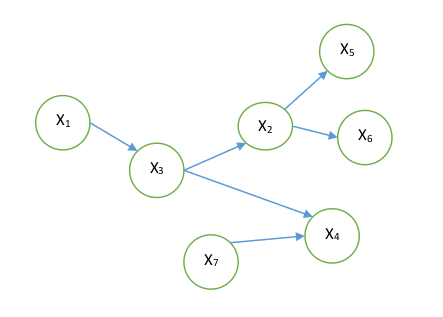
\includegraphics[width=0.5\textwidth]{4}
\caption{شکل سوال دوم}
\label{fig1}
\end{figure}

\subsubsection{توزیع توام}

$P(X_1, \dots , X_7) = P(X_1)P(X_3 \ | \ X_1)P(X_2 \ | \ X_3)P(X_5 \ | \ X_2)P(X_6 \ | \ X_2)P(X_4 \ | \ X_3 , X_7)P(X_7)$

\subsubsection{درستی و نادرستی}

\begin{itemize}
\item{$X_1 \perp X_5 \ | \ X_2 $}:
درست است. اگر 
$X_2$
را بدانیم مسیر فعال بین $X_1$ و $X_5$ غیر فعال می‌شود و مستقل می‌شوند.
\item{$X_2 \perp X_7 \ | \ X_4 $}:
نادرست است. در ساختار وی-شکل بین $X_7$ و $X_3$ با دانستن $X_4$ وابستگی ایجاد می‌شود، و چون $X_2$ به پدرش $X_3$ وابسته است، با $X_7$ نیز در این شرایط وابسته است. 

\item{$X_1 \perp X_5 \ | \ X_2 $}:
درست است، چرا که دانستن $X_3$ ، استقلال بین $X_2$ و $X_4$ را ایجاد می‌کند و بنابر این از فرزندان $X_2$ یعنی $X_5$ نیز مستقل می‌شویم. 

\subsubsection{ \lr{Markov Blanket for $X_3$} }
برای این کار ابتدا جهت‌ها را حذف می‌کنیم و سپس فساد\LTRfootnote{ Immorality} ها را حذف می‌کنیم. یعنی نباید گره‌ای باشد که والد یکی از فرزندان همین گره باشد، در صورت وجود به آن گره وصل می‌کنیم تا فساد از بین برود. به تمامی اتصالات موجود نیز وصل می‌کنیم، بنا بر این
$MB(X_3) = \lbrace X_1 , X_2 , X_4 , X_7 \rbrace $
خواهد بود. 
\end{itemize}

\section{بخش پیاده‌سازی}

\subsection{مقدمه}
در این بخش باید با استفاده از پایگاه داده‌ی معرفی شده، چند مدل‌ بیزین ارایه کنیم تا قادر به تشخیص بیماری قلبی باشد. 

برای پیاده‌سازی این بخش، تصمیم به توسعه‌ی ابزار جدیدی برای کار با مدل‌های احتمالاتی گرافیکی گرفتیم، که کاملا با ابزارهای تحت خط فرمان سیستم‌عامل لینوکس و پوسته‌ی \lr{Bash} کار می‌کند. این‌گونه ابزارها، معمولا برای استفاده در مواردی که فایل‌های حجیمی نیاز به پردازش دارند و می‌خواهیم درگیر مسایل مدیریت حافظه و \lr{Caching} نشویم کاربرد دارند. همچنین، دید مبتنی بر فایل در بسیاری موارد به کمک توسعه‌دهنده می‌آید و توسعه‌ی ابزارها تحت قالب \lr{Shell Script}، انعطاف بسیار زیادی را برای برنامه‌نویس فراهم می‌کند. این گونه ابزارها معمولا در فازهای یادگیری به دلیل نیاز به نوشتن مفرط در فایل کند هستند، به‌گونه‌ای که ابزار تولید شده در این تمرین عملا کارایی برای آموزش روی داده‌ها ندارد که در تمرینات آتی به رفع این ایرادها می‌پردازیم. در عوض، از آن‌جا که به کل مساله‌ی آموزش و تست به دید مساله‌ی پردازش متن نگاه کرده‌ایم، در فاز تست سرعت پاسخ‌گویی بسیار بالا خواهد بود چرا که ابزارهای پروژه‌ی \lr{GNU} مانند \lr{grep} که برای جست‌وجو استفاده می‌شوند و یا \lr{awk}، \lr{sed} و \lr{cut} که به دفعات بسیاری از آن‌ها استفاده نموده‌ایم، کارایی به شدت بالایی در پردازش فایل‌های عظیم دارند. به این ترتیب در پردازش پایگاه‌های داده‌ی بیش از حد بزرگ و زمانی که \lr{CPD} ها بزرگ می‌شوند و نیاز به جست‌وجوی موثر داریم، کارا خواهند بود. همچنین انعطاف در تعیین نوع داده‌ای ویژگی‌ها و متغیرها از جمله‌ مزیات دیگر این ابزار است و ورودی و خروجی‌های تولید شده به آسانی با دیگر ابزارهای تحت خط فرمان لینوکس قابل استفاده هستند. 

در ادامه پس از توضیح چگونگی استفاده از پایگاه داده، به بررسی ابزار توسعه داده‌شده و پاسخ سوالات تمرین می‌پردازیم. 
{\large{\frownie}}

\subsection{پایگاه داده و پردازش ها}

با دریافت پایگاه‌ داده‌ی شهر کلیولوند\LTRfootnote{ Cleveland} از سایت معرفی شده
\LTRfootnote{ \url{http://archive.ics.uci.edu/ml/datasets/Heart+Disease}}
، به بررسی ستون‌های ویژگی و پردازش‌های مورد نیاز پرداختیم. آزمایش‌ها بر روی نسخه‌ی تجدیدنظر شده نیز انجام گرفتند
\LTRfootnote{ \url{http://archive.ics.uci.edu/ml/machine-learning-databases/statlog/heart/}}
. از جمله گسسته‌سازی هر ویژگی با توجه به مفاهیم آن انجام گرفت، در زیر توضیحات گسسته‌سازی آورده شده است: 
\begin{enumerate}
\item{\textbf{سن}}: 
این متغیر با مقادیر گسسته‌ی ۲،۳،۴،۵،۶ و ۷ نمایش‌ داده‌شد، تا نشان‌دهنده‌ی رقم دهگان نمونه‌ی مورد نظر باشد.

\item{\textbf{کلسترول}}: 
مقادیر کمتر از ۲۰۰ (سالم) ، بین ۲۰۰ تا ۲۴۰ (مرز سلامتی) و بالاتر از ۲۴۰ (خطرناک) به ترتیب با اعداد ۱، ۲ و ۳ نشان داده شدند\LTRfootnote{ \url{http://en.wikipedia.org/wiki/Cholesterol}}. 

\item{\textbf{فشار خون در استراحت}}: 
به ترتیب در بازه‌های ۹۰-۱۱۹، ۱۲۰-۱۳۹، ۱۴۰-۱۵۹، ۱۶۰-۱۷۹ و بیش از ۱۸۰ در نظر گرفته شدند و اعداد یک تا پنج به آن‌ها اختصاص داده‌شد
\LTRfootnote{ \url{http://en.wikipedia.org/wiki/Blood_pressure}}
.
\item{\textbf{\lr{Old Peak}}}: 
با توجه به بازه‌های موجود در پایگاه، بازه‌های صفر تا یک، یک تا دو، دو تا سه، سه تا پنج و پنج تا ۷ در نظر گرفته شدند. 
\item{\textbf{بیشینه ضربان قلب}}: 
برای محاسبه‌ی این ویژگی، سن طبق فرمول‌های زیادی از جمله :
$$208 - (0.7 * \text{سن} )$$
تاثیر دارد
\LTRfootnote{ \url{http://en.wikipedia.org/wiki/Heart_rate\#Maximum_heart_rate}}
. 
با محاسبه‌ی این اعداد برای سنین ۲۰ تا هفتاد سالگی، به اعداد نرمال برای این ویژگی رسیدیم و بازه‌های زیر را در نظر گرفتیم : 

کمتر از ۱۵۹، تا ۱۶۶، تا ۱۷۳، تا ۱۸۰، تا ۱۸۷، تا ۱۹۴، و بالاتر از ۱۹۴ که هفت دسته را شامل می‌شود.
\item{\textbf{حضور بیماری}}: 
در پایگاه‌داده‌ی قدیمی‌تر، مقادیر غیر صفر و ناشناخته را دو در نظر گرفتیم که نشان وجود بیماری است و یک عدم وجود آن. 

\end{enumerate}

به جای مقادیر ناشناخته، مقادیر میانگین هر ستون را قرار دادیم، این اعمال با دو اسکریپت توسعه داده شده تحت نام‌های \lr{changeUnknownWithMean.sh} و \lr{quantizeQuery.sh} (که برای یک خط کار می‌کند و روی کل خطوط فایل داده فراخوانی می‌شود) انجام می‌گیرد. همچنین برای اطمینان از این که سطرهای پایگاه داده هم طول هستند می‌توانید از اسکریپت \lr{checkLines.sh} استفاده کنید.


\subsection{ابزارهای توسعه‌داده شده و ساختار}

در این ابزار، ابتدا نیاز دارید با دو اسکریپت معرفی شده در بخش قبل فایل مورد نظر را بسازید، از این پس به نام پایگاه داده از این فایل گسسته‌سازی شده یاد می‌کنیم و ابزارهای توسعه‌ داده‌ شده‌ی مرتبط نیز در بخش قبل معرفی شد. سپس باید متغیرهای تصادفی خود را و این که هر کدام در چه ستونی از پایگاه داده هستند در یک فایل مانند \lr{vars.define} مانند زیر با دو نقطه و در هر خط معرفی کنید:

\begin{latin}
\noindent
age:1\\
sex:2\\
chest:3\\
RBP:4\\
chol:5\\
FBS:6\\
RC:7\\
MHR:8\\
EIA:9\\
oldPak:10\\
slope:11\\
vessels:12\\
thal:13\\
HD:14\\
\end{latin}

دقت کنید که این فایل باید به ترتیب عددی ستون‌ها از بالا به پایین مرتب شده باشد در غیر این صورت الگوریتم‌های آتی دچار مشکل خواهد شد. 


رعایت تمامی نکات دستوری بالا و آنچه در ادامه خواهد آمد لازم است چرا که تمامی پردازش‌ها با این فرض انجام شده است.

سپس نیاز دارید بازه‌های داده‌ها را استخراج کنید که در اصل مقادیر مجاز برای داده‌ها می‌باشند. این کار را می‌توانید با اسکریپت توسعه‌داده شده با نام \lr{extractRanges.sh} انجام دهید، مانند: 

\lr{./extractRanges.sh ../Dataset/cleveland-bin.quantized ./Sample/vars.define ./Sample/newVars/}

که پارامتر اول پایگاه داده، دوم فایل توصیف متغیرها و سومی مکانی برای ساخت بازه‌های متغیرها است. این نحوه آدرس‌دهی را در اکثر اسکریپت‌های توسعه‌داده شده خواهید دید. پس از اجرا، در آدرسی که برای ساخت بازه‌های متغیرها دادیم، 
فایل‌هایی با پسوند \lr{.var} ساخته می‌شود که در آن مقادیر مجاز با کاما از هم جدا شده‌اند. به نفع کاربر است که در مقادیر متغیرها از فاصله یا \lr{wildchar}ها مانند ستاره استفاده نکند چرا که در عملیات دستوری ممکن‌ است خطاهای ناخواسته ایجاد شود.

پس از این، نوبت به ساخت معماری شبکه‌ی مورد نظر می‌رسد. برای این کار ساختار ساده‌ای در نظر گرفتیم، در یک فایل به ازای هر یال پدر به فرزند، یک زوج متغیر با فاصله از هم جدا می‌شوند، مانند زیر که نمونه یک شبکه‌ی \lr{Naïve Bayes} برای ۹ متغیر ویژگی و یک متغیر کلاس بیماری است که با نام \lr{myBn.bn} ذخیره شده است. دقت کنید پسوند فایل‌های معرفی شده مهم نمی‌باشد. 
\begin{latin}
\noindent
HD age\\
HD sex\\
HD chest\\
HD RBP\\
HD chol\\
HD FBS\\
HD RC\\
HD MHR\\
HD EIA\\
HD oldPak\\
HD slope\\
HD vessels\\
HD thal\\
\end{latin}

برای آموزش شبکه‌ی معرفی شده، اسکریپت \lr{train.sh} را به صورت زیر صدا کنید (اسامی برای مثال آورده شده‌اند):


{\footnotesize{\lr{./train.sh Sample/vars.define ../Dataset/cleveland-bin.quantized ./Sample/naiveBayes.bn ./Sample/varsNaive/}}}

این اسکریپت، از ماژول‌های زیرین کوچک‌تری استفاده می‌کند که هر کدام وظایف اتمیک در مدل‌های احتمالاتی را دارند، برای نمونه ساخت جداول \lr{CPD} یکی از این ماژول‌ها است و یا با اسکریپت \lr{probQuery.h} می‌توان مستقیما احتمال یک پیشامد را با نام متغیرها و مقادیر آن‌ها در جدول‌های احتمال توام جست‌و‌جو کرد. همچنین پس از ساخت \lr{CPD} ها می‌توان یک احتمال شرطی را با اسکریپت \lr{cpdQuery.sh} از پایگاه سوال کرد. 

پس از اجرای اسکریپت \lr{train.sh} دو پوشه در مسیر جاری به نام‌های \lr{joints} و \lr{CPD} ساخته می‌شوند. فایل‌های پوشه‌ی اول جداول توام ساخته شده از روی پایگاه هستند که پسوند \lr{.joint} دارند و در پوشه دوم، \lr{CPD} ها با پسوند \lr{visualized} قابل دسترسی هستند، هرچند سیستم طراحی شده از جداول با پسوند \lr{.cpd} استفاده می‌کند که به دلیل ذخیره‌سازی خطی، برای خواندن در خط فرمان و جست‌و‌جو ساده‌تر هستند. یکی از ابزارهای دیگر، ابزاری سریع برای تولید انواع ترکیب‌های متغیرهای ورودی است که \lr{combineVars.sh} نام‌ دارد و برای ساخت مقادیر ممکن برای سطرهای جداول توام و شرطی به کار می‌رود. 

اسکریپت \lr{leaveOneOut.sh} نیز از اسکریپت \lr{train.sh}، \lr{makeNthQuery.sh} که عمل یک خط خاص را جدا کردن و کوئری ساختن از آن را برایمان انجام می‌دهد، و \lr{fullObserveQuery.sh} یک کوئری ساده‌ برای کلاس به شرط مشاهدات (همه متغیرها) را انجام می‌دهد. این کار برای ناییو بیز به سادگی از فرمول :

\begin{equation}
P(Y=y \ | \ E = e ) = { {P(E \ | \ Y) \cdot P(Y) } \over {\sum_{y} P(E \ | \ Y_y)P(Y_y)} }
\end{equation}

محاسبه‌ی این مقدار با توجه به مستقل بودن به شرط دانستن \lr{Y} در ناییو بیز، در اسکریپت \lr{fullObserveQuery.sh} پیاده‌سازی شده‌است. 

متاسفانه این ابزار هنوز برای همه‌ی مدل‌ها پاسخ‌گو نیست چرا که نیاز به پیاده‌سازی روش‌های استنتاج دارد و پیچیدگی‌های فنی بسیار زیاد \lr{Shell Script} روند کار را به شدت کند می‌کند. برای این تمرین در حد آموزش و تست ناییو بیز نتایج درست است ولی در شبکه‌های دیگر درست کار نمی‌کند که از آوردن نتایج آن خودداری کرده‌ایم، چرا که تا توسعه نیافتن ابزار استنتاج ارزشی نخواهد داشت. از مزیت‌های این ابزار انجام محاسبات تا ۲۱ رقم اعشار است که در زیاد بودن تعداد پارامترها به ما کمک می‌کند، هر چند برای سهولت بیشتر در خواندن اعداد، این ارقام را تا نه رقم اعشار چاپ کرده‌ایم. 

\subsection{نتایج}

نتایج اجرای \lr{Leave one out} برای دو پایگاه داده شهر کلیولند بررسی شدند. در ابتدا هر دو پایگاه در یک شبکه ناییو بیز با ۱۴ پارامتر تست شدند که نتایج در زیر آورده شده است. تعداد تشخیص‌های درست را در تصویر مشاهده می‌کنید. 

\begin{figure}[h]
\centering
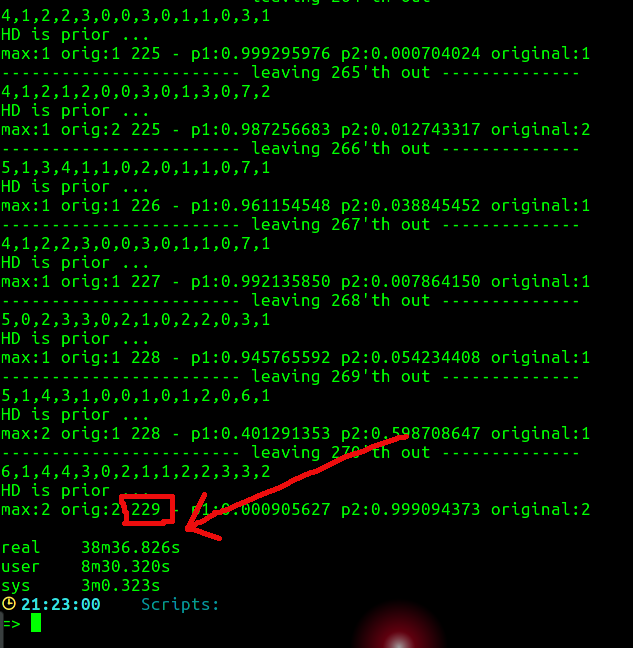
\includegraphics[width=0.5\textwidth]{1}
\caption{نتایج برای پایگاه‌داده نسخه جدید با ۱۴ ویژگی - ناییو بیز}
\label{fig2}
\end{figure}

مشاهده می‌کنید که به دلیل استفاده از حلقه‌های متعدد در اسکریپت‌ها، زمان اجرای \lr{Leave one out} عملا غیر قابل کاربرد است (نزدیک به ۳۰ دقیقه) که ضعف اصلی ابزار توسعه داده شده می‌باشد. هرچند انتظار می‌رود با استفاده از یک فایل سیستم \lr{tmpfs} که از حافظه اصلی \lr{RAM} برای ذخیره‌سازی استفاده می‌کند کمی بهبود یابد اما امیدی به کارایی بالا در استنتاج‌های پیچیده‌تر نیست. 

برای پایگاه داده‌ی نسخه‌ی جدید، با ۱۴ متغیر، دقت
$0.84814814814814814814$
و با پایگاه قدیمی که مقادیر ناقص آن با میانگین ستون‌ها جاگزین شد دقت 
$0.92592592592592592592$
حاصل شد. برای آزمون، با توجه به جداول \lr{CPD} در همین مدل‌ها، آن دسته ویژگی‌هایی که احتمال‌هایشان یک‌نواخت تر توزیع شده بود و اعدادشان برای دسته‌های متفاوت نزدیک به هم بود، کنار گذاشته شد (متغیرهای 
\lr{RBP,FBS,RC,oldPeak})
و دوباره تست انجام گرفت. دقت‌ها به ترتیب برای پایگاه جدید با اندکی کاهش به 
$0.84074074074074074074$
رسید ولی برای پایگاه قدیمی ثابت ماند. بنابراین استفاده از پایگاه داده‌ی قدیمی دقت بیشتری به دست داد. هرچند روش درست حل این مساله، ترتیب اثر دادن ماتریس هزینه برای تشخیص غلط بیماری است که باید به جای بیشترین احتمال، مجموع هزینه (احتمال ضرب در هزینه) روی همه‌ی پیش‌بینی‌های موجود محاسبه شود و آن پیش‌بینی که این هزینه را کمینه می‌کند انتخاب شود که متاسفانه در این فاز از تمرین به انجام نرسید. 





















\end{document} 
